% arara: pdflatex: { draft: yes }
% arara: bibtex
% arara: pdflatex: { draft: yes }
% arara: lualatex: {
% arara: --> shell: yes,
% arara: --> synctex: yes,
% arara: --> interaction: batchmode
% arara: --> }
% arara: clean: {
% arara: --> extensions:
% arara: --> ['log','aux','out','pytxcode','synctex.gz','toc','bbl','bcf','blg', 'abs','out']
% arara: --> }
%% 
%% Copyright 2019 Elsevier Ltd
%% 
%% This file is part of the 'CAS Bundle'.
%% --------------------------------------
%% 
%% It may be distributed under the conditions of the LaTeX Project Public
%% License, either version 1.2 of this license or (at your option) any
%% later version.  The latest version of this license is in
%%    http://www.latex-project.org/lppl.txt
%% and version 1.2 or later is part of all distributions of LaTeX
%% version 1999/12/01 or later.
%% 
%% The list of all files belonging to the 'CAS Bundle' is
%% given in the file `manifest.txt'.
%% 
%% Template article for cas-dc documentclass for 
%% double column output.

%\documentclass[a4paper,fleqn,longmktitle]{cas-dc}
\documentclass[a4paper,fleqn]{cas-dc}
\usepackage{mathtools}
\usepackage{dsfont,bm}
\usepackage[authoryear,longnamesfirst]{natbib}
%\usepackage[authoryear]{natbib}
%\usepackage[numbers]{natbib}

%%%Author definitions
\def\tsc#1{\csdef{#1}{\textsc{\lowercase{#1}}\xspace}}
\tsc{QE}
\tsc{EP}
\tsc{PMS}
\tsc{BEC}
\tsc{DE}
%%%
\newtheorem{theorem}{Teorema}
\renewcommand{\figurename}{Figura}
\renewcommand{\tablename}{Tabla}

\begin{document}
\let\WriteBookmarks\relax
\def\floatpagepagefraction{1}
\def\textpagefraction{.001}
\shorttitle{Aplicaciones de la función Cobb-Douglas}
\shortauthors{C. Torres Ponce et~al.}

\title [mode = title]{Las aplicaciones de la función de producción Cobb-Douglas en la industria}
\tnotemark[1]%,2

\tnotetext[1]{Este documento es el resultado de la investigación del proyecto financiado por la Fundación de Matemática de la Facultad de Ciencias.}

%\tnotetext[2]{La nota al pie del segundo título, que es un texto más largo
%	para llenar todo el ancho del texto y desbordar en
%	otra línea en el área de notas al pie de la primera página.}



\author[1,2]{C. Torres Ponce}[type=editor,
                        auid=000,bioid=1,
                        prefix=Sir,
                        role=Investigador,
                        orcid=0000-0002-3746-252X]
\cormark[1]
%\fnmark[1]
\ead{ctorresp@uni.edu.pe}

\credit{Conceptualization of this study, Methodology, Software}

\address[1]{Facultad de Ciencias - Escuela Profesional de Matemática}

\author[1,2]{C. Aznarán Laos}[%
style=chinese,
role=Coordinador,
orcid=0000-0001-8314-2271
]
\cormark[2]
\ead{caznaranl@uni.pe}
\ead[URL]{https://carlosal1015.github.io/}
\cortext[cor1]{Autor correspondiente}
\cortext[cor2]{Autor principal correspondiente}

\author[2,3]{K. Fernández Huidobro}
\ead{kfernandezh@uni.pe}
\cormark[1]

\credit{Data curation, Writing - Original draft preparation}

\address[2]{Facultad de Ciencias - Escuela Profesional de Ciencia de la Computación}

\author[2,3]{B. Torres Ayalas}
\ead{btorresa@uni.pe}
\cormark[1]
\author[2,3]
{A. Berrospi Casano}[style=chinese]
\ead{aberrospic@uni.pe}
\cormark[2]

\address[3]{Universidad Nacional de Ingeniería, Av. Túpac Amaru 210, Rímac, Lima 25, Perú}

%\fntext[fn1]{This is the first author footnote. but is common to third
%  author as well.}
%\fntext[fn2]{Another author footnote, very long footnote and
%  it should be a really long footnote. But this footnote is not yet
%  sufficiently long enough to make two lines of footnote text.}

%\nonumnote{This note has no numbers. In this work we demonstrate $a_b$
%	the formation Y\_1 of a new type of polariton on the interface
%	between a cuprous oxide slab and a polystyrene micro-sphere placed
%	on the slab.
%}

\begin{abstract}
This

\noindent A
\end{abstract}

\begin{graphicalabstract}
\centering
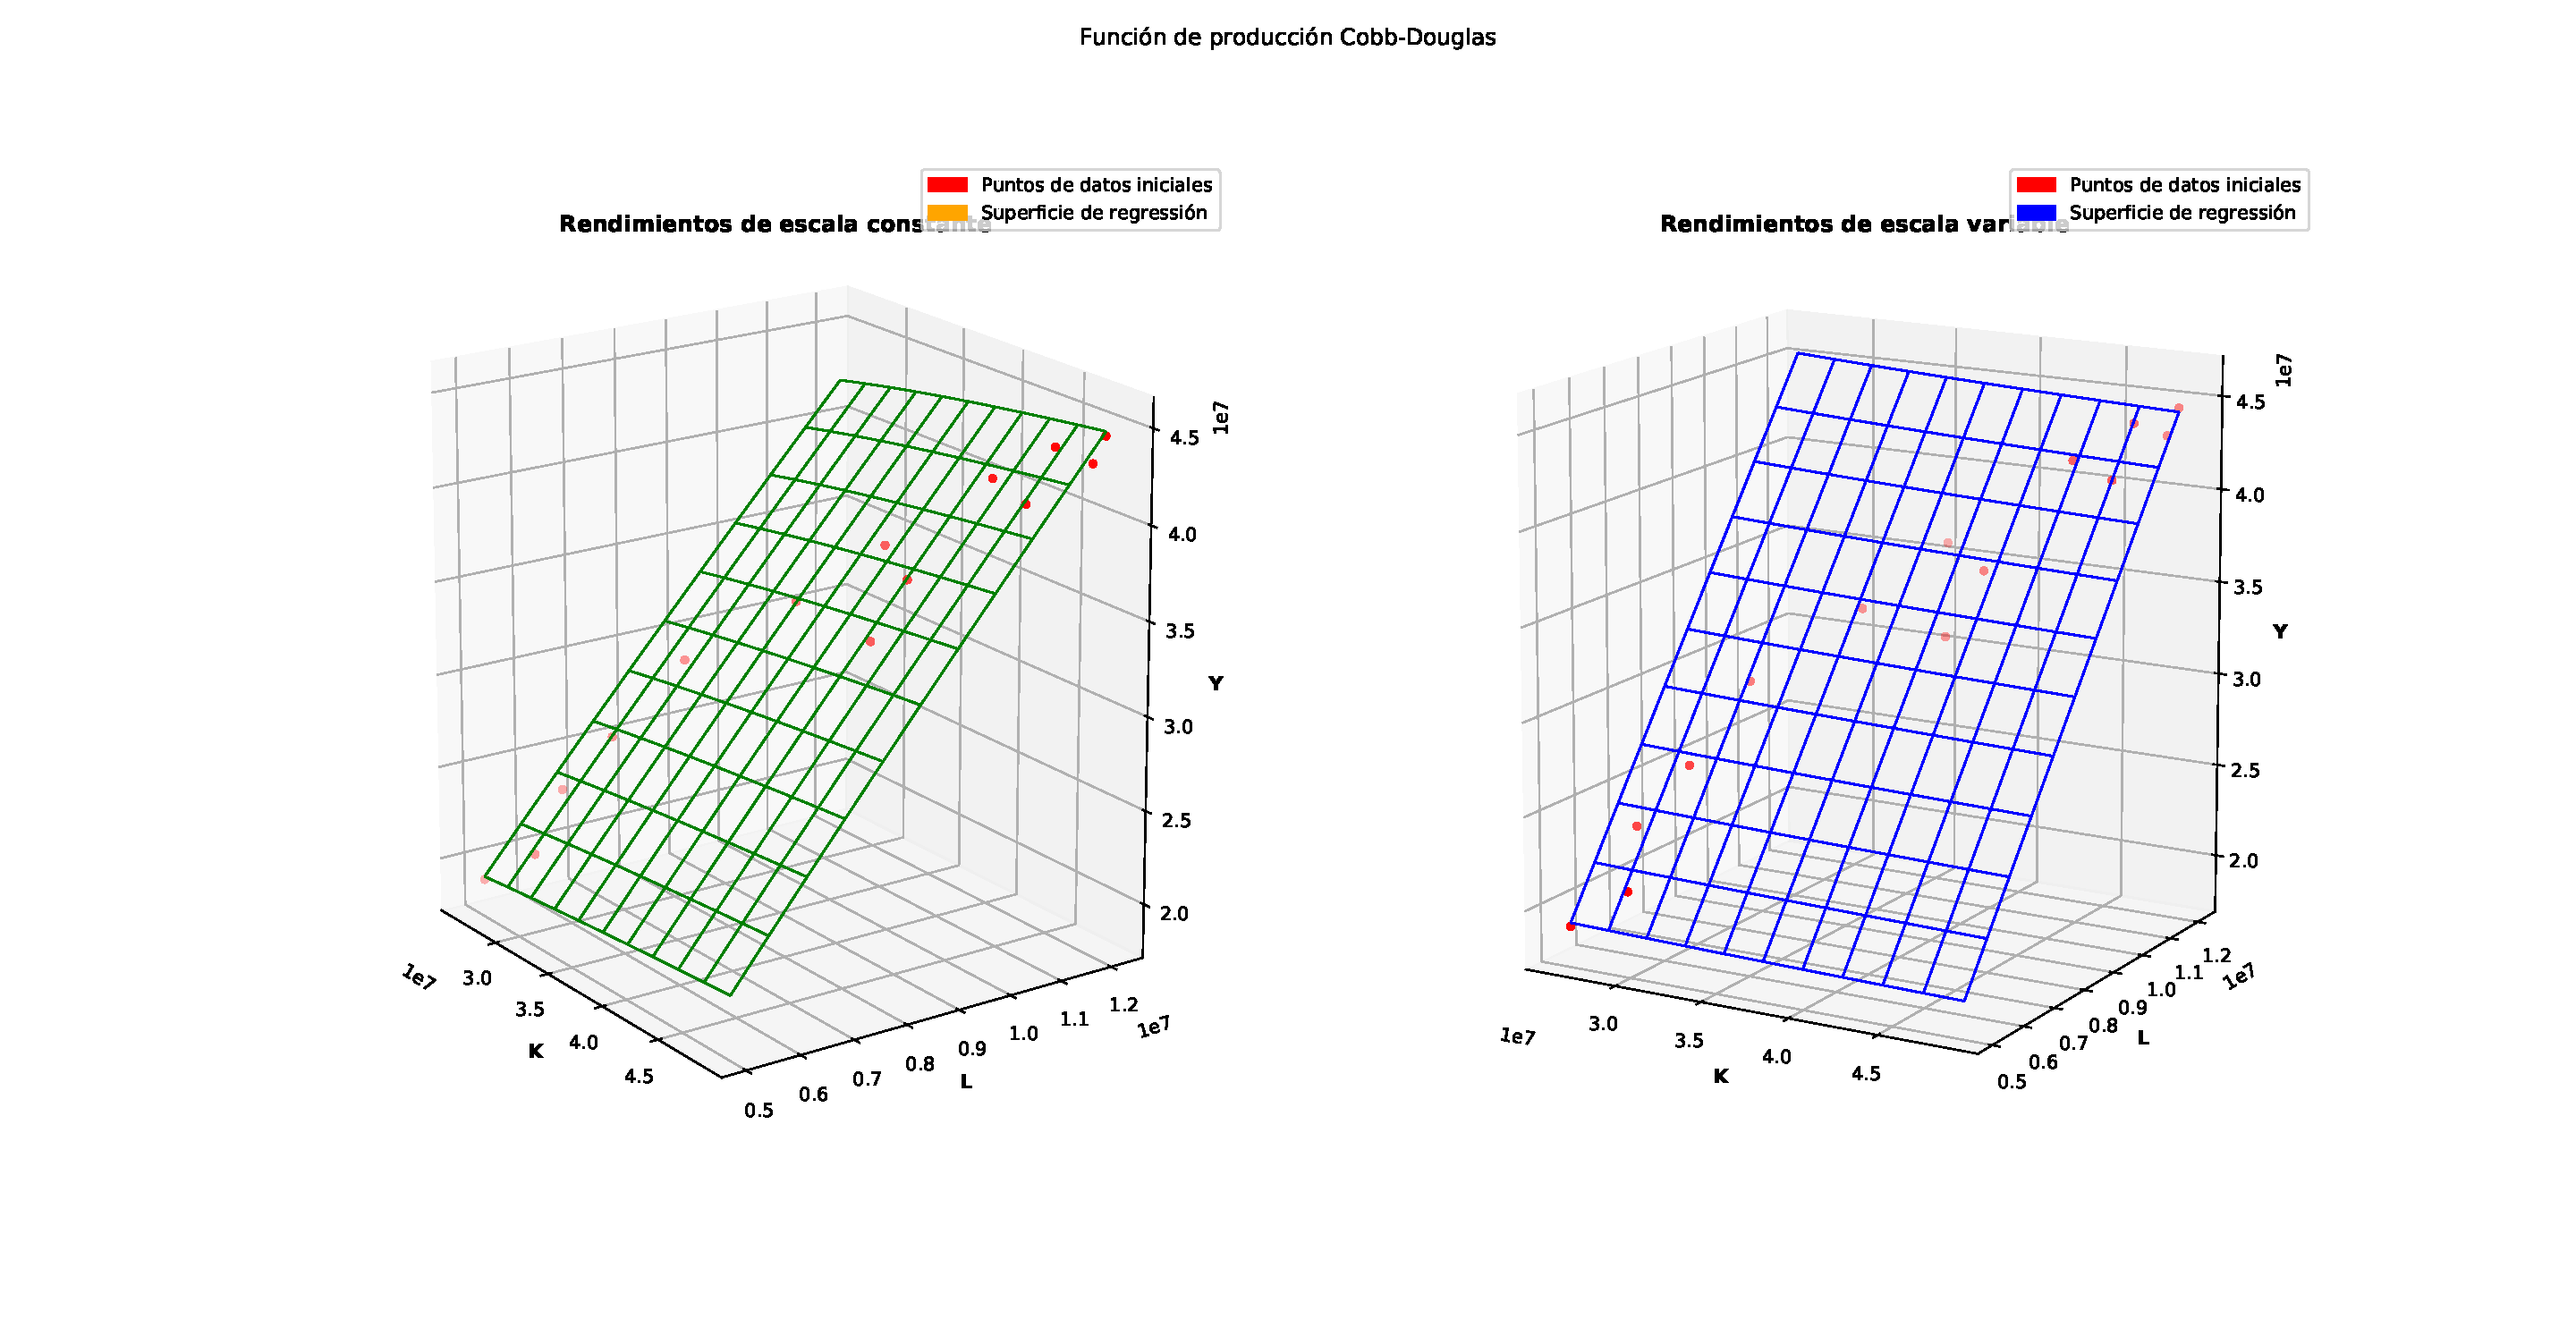
\includegraphics[width=0.9\paperwidth]{figs/withnaturalog.pdf}\\
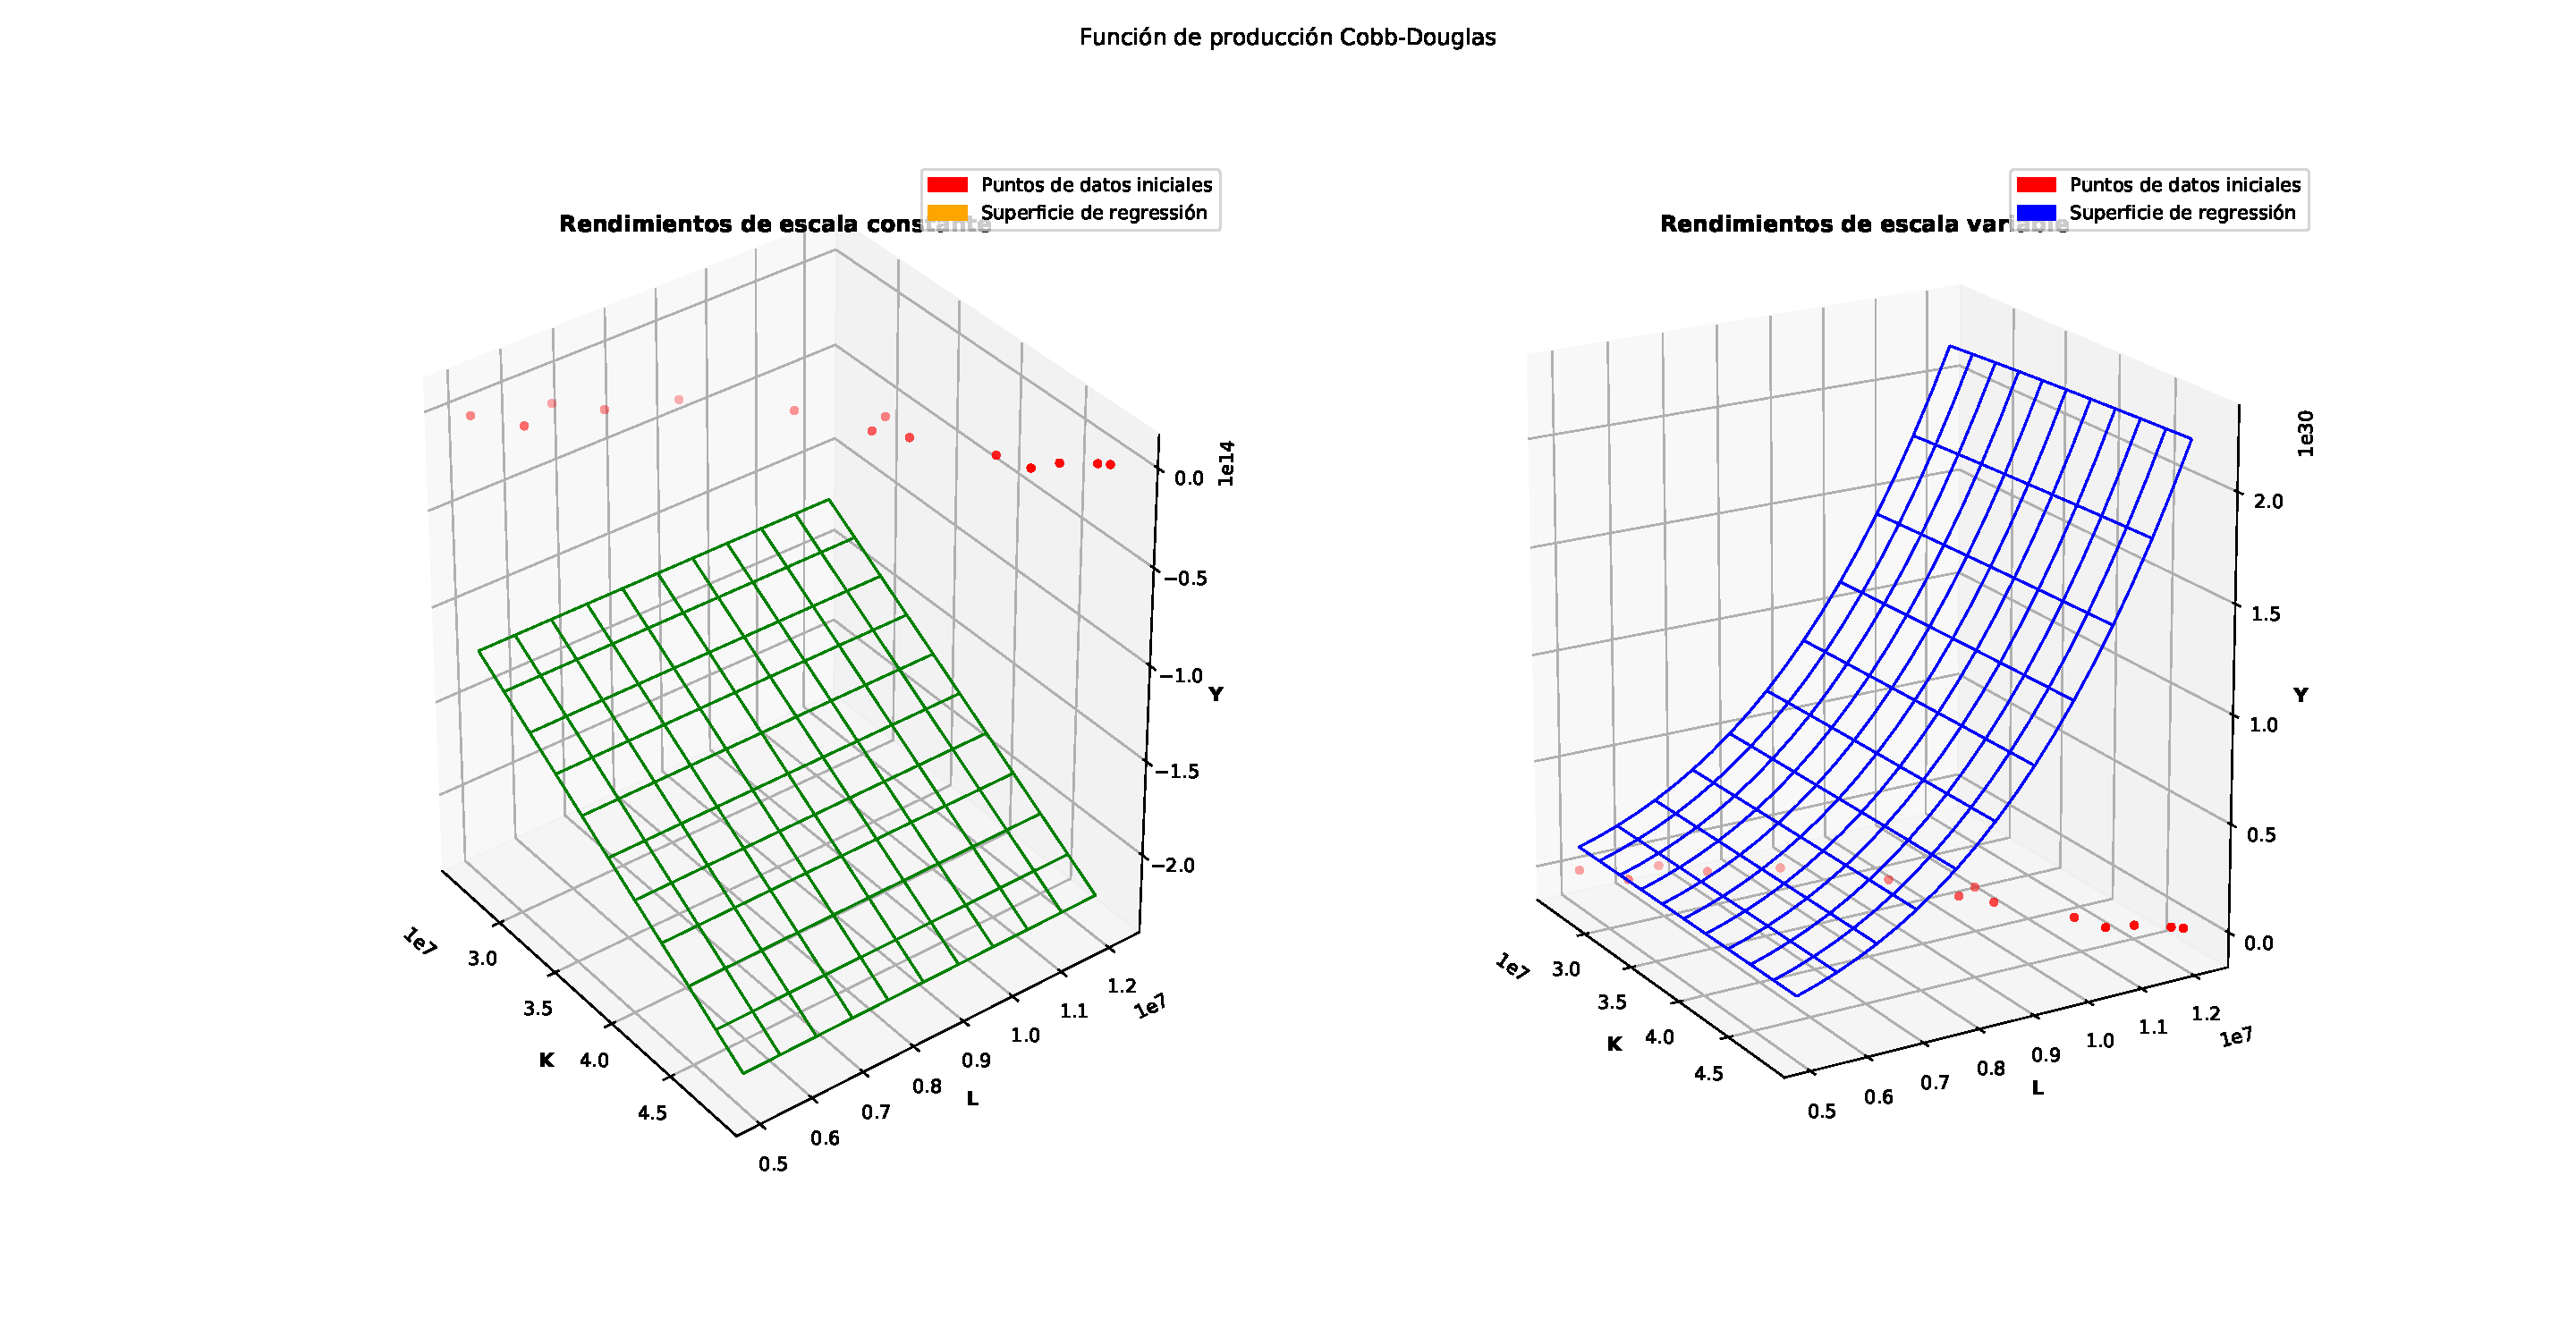
\includegraphics[width=0.9\paperwidth]{figs/withoutnaturalog.pdf}
\end{graphicalabstract}

\begin{highlights}
\item Modelo de crecimiento económico de Solow-Swan (1940).
\item Modelo de crecimiento económico de Ramsey (1920).
\end{highlights}

\begin{keywords}
Cobb-Douglas \sep \BEC
\end{keywords}

\maketitle

\section{Introducción}
En economía, una función de producción es una función que especifica la máxima salida posible de una empresa, industria o una economía entera  para todas las posibles entradas. En general, una función de producción puede darse como $y=f\left(x_{1},x_{2},\ldots,x_{n}\right)$ donde $y$ es la cantidad de salida, $x_{1},x_{2},\ldots,x_{n}$ son las entras de factores de producción (tales como el capital, trabajo, tierra o materias primas). No permitiremos la producción conjunta, es decir, los procesos de producción, los cuales tienen múltiples coproductos o salidas. Por supuesto ambas entradas deben ser positivas. Sobre la historia de las funciones de producción mire el trabajo. Varios aspectos de las funciones de producción se tratan en la monografía.

Sean $\mathds{R}$ y $\mathds{R}_{+}$ los conjuntos de números reales y números reales positivos, respectivamente.
\newtheorem{definition}{Definición}

\begin{definition}
Una función $f\colon\mathds{R}^{n}_{+}\rightarrow\mathds{R}_{+}$ es llamada una \textbf{función de producción}.
\end{definition}
A continuación, asumimos que las funciones de producción son dos veces continuamente diferenciables. La elasticidad de sustitución fue introducida originalmente por J. R. Hicks (1932) [10] (en el caso de dos entradas) con el propósito de analizar los cambios en la participación de los ingresos del trabajo y el capital. R. G. D. Allen y J. R. Hicks (1934) [3] sugirieron dos generalizaciones del concepto original de elasticidad variable de Hicks. El primer concepto que llamamos elasticidad de sustitución de Hicks se define como sigue.
\begin{definition}
Sea $f\colon\mathds{R}^{n}_{+}\rightarrow\mathds{R}_{+}$ una función de producción con primeras derivadas parciales no nulas. La función
\begin{equation}
H_{ij}\left(\bm{x}\right)=-\frac{\frac{1}{x_{i}f_{i}}+\frac{1}{x_{j}f_{j}}}{\frac{f_{ii}}{{\left(f_{i}\right)}^{2}}-\frac{2f_{ij}}{f_{i}f_{j}}+\frac{f_{jj}}{{\left(f_{j}\right)}^{2}}}\quad\left(\bm{x}\in\mathds{R}^{n}_{+},i,j=1,\ldots,n,i\neq j\right)
\end{equation}
donde los subíndices de $f$ denotan las derivadas parciales, es decir, $f_{i}=\frac{\partial f}{\partial x_{i}}$, $f_{ij}=\frac{\partial^{2}f}{\partial x_{i}\partial x_{j}}$, todas las derivadas son tomadas en el punto $\bm{x}$ y el denominador es asumido distinto de cero) es llamada la \textbf{elasticidad de sustitución de Hick} de la $i$--ésima variable (factor) de producción con respecto a la $j$--ésima variable (factor) de producción.
\end{definition}
El otro concepto () %TODO
\begin{definition}
Sea $f\colon\mathds{R}^{n}_{+}\rightarrow\mathds{R}_{+}$ una función de producción. La función
\begin{equation}
A_{ij}\left(\bm{x}\right)=-\frac{x_{1}f_{1}+x_{2}f_{2}+\cdots+x_{n}f_{n}}{x_{i}x_{j}}\frac{F_{ij}}{F}\quad\left(\bm{x}\in\mathds{R}^{n}_{+},i,j=1,\ldots,n,i\neq j\right)
\end{equation}
donde $F$ es el determinante de la matriz confinada
\begin{equation}
M=
\begin{bmatrix}
0 & f_{1} & \cdots & f_{n}\\
f_{1} & f_{11} & \cdots & f_{1n}\\
\vdots & \vdots & \cdots & \vdots\\
f_{n} & f_{n1} & \cdots & f_{nn}
\end{bmatrix}
\end{equation}
y $F_{ij}$ es el cofactor del elemento $f_{ij}$ en el determinante $F$ ($F\neq0$ es asumida y todas las derivadas son tomadas en el punto $\bm{x}$) es llamada la \textbf{elasticidad de sustitución de Allen} de la $i$--ésima variable (factor) de producción con respecto a la $j$--ésima variable (factor) de producción.
\end{definition}

\begin{definition}
Una función dos veces diferenciable $f\colon\mathds{R}^{n}_{+}\rightarrow\mathds{R}_{+}$ se dice que satisface la \textbf{propiedad CES} (elasticidad de sustitución constante) si existe una constante $\sigma\in\mathds{R}$, $\sigma\neq0$ tal que
\begin{equation}
H_{ij}\left(\bm{x}\right)=\sigma\quad\left(\bm{x}\in\mathds{R}^{n}_{+},i,j=1,\ldots,n,i\neq j\right).
\end{equation}
\end{definition}
En la secuela discutimos que hasta qué punto la propiedad CES (4) determina la función de producción.

C.W. Cobb y P.H. Douglas [6] estudiaron cómo la distribución de los ingresos nacionales pueden describirse con ayuda de las funciones de producción. El resultado de su estudio fue la función de producción \[ f\left(\bm{x}\right)=Cx^{\alpha_{1}}_{1}\cdots x^{\alpha_{n}}_{n}\quad\left(\bm{x}\in\mathds{R}^{n}_{+}\right) \] donde $C>0$, $\alpha_{i}\neq0$ $\left(i=1,\ldots,n\right)$ son constantes satisfaciendo $\alpha\coloneqq\sum_{i=1}^{n}\alpha_{i}\neq0$. Llamaremos esta \textbf{función de producción Cobb-Douglas (o CD)}.

En 1961, K.J.Arrow, H.B.Chenery, B.S.Minhas y R.M.Solow introdujo una nueva función de producción. \[ f\left(\bm{x}\right)={\left(\beta_{1}x_{1}^{\frac{m}{\beta}}+\cdots+\beta_{n}x_{n}^{\frac{m}{\beta}}\right)}^{\beta}\quad\left(\bm{x}\in\mathds{R}^{n}_{+}\right) \] donde $\beta_{i}>0$ $\left(i=1,\ldots,n\right)$, $m\neq0$, $\beta\neq0$ son constantes reales. Nos referiremos a la función \textbf{Arrow-Chenery-Minhas-Solow} o (ACMS) \textbf{función de producción}.

Las funciones de producción CD y ACMS tienen la misma propiedad, llamemoslo así como fácil de verificar $H_{ij}=1$ para la funciones CD y $H_{ij}=\frac{1}{1-\frac{m}{\beta}}$ para las funciones de producción AMCS si $\frac{m}{\beta}\neq1$, para $\frac{m}{\beta}=1$ el denominador de $H_{ij}$ es cero, por lo tanto, este no está definido.

\begin{definition}
	Una función $F\colon\mathds{R}^{n}_{+}\rightarrow\mathds{R}_{+}$ es llamada \emph{homogénea de grado} $m\in\mathds{R}$ si \[ F\left(t\bm{x}\right)=t^{m}F\left(\bm{x}\right) \] se cumple para $\bm{x}\in\mathds{R}^{n}_{+}$, $t>0$.
\end{definition}

\begin{definition}
Una función $F\colon\mathds{R}^{n}_{+}\rightarrow\mathds{R}_{+}$ es llamada \emph{subhomogénea de grado} $m\in\mathds{R}$ si \[ F\left(t\bm{x}\right)\leq t^{m}F\left(\bm{x}\right) \] se cumple para todo $\bm{x}\in\mathds{R}^{n}_{+}$ y para todo $t>1$. La función $F$ es llamada \emph{superhomogénea de grado} $m\in\mathds{R}$ si la desigualdad inversa se cumple.
\end{definition}

Las funciones homogéneas (sub y superhomogéneas) de grado $1$ simplemente se llamarán funciones homogéneas (sub y superhomogéneas).

Si $F$ es una función de producción, entonces en economía también los términos rendimientos a escala constantes, rendimientos a escalas decrecientes y crecientes son usados para designar la homogeneidad, subhomogeneidad y superhomogeneidad de las funciones (de producción), respectivamente.

Es bien conocido que las funciones $F$ diferenciables homogéneas de grado $m$ puede ser caracterizados por la ecuación en derivadas parciales de Euler \[ x_{1}F_{x_{1}}\left(\bm{x}\right)+\cdots+x_{n}F_{x_{n}}\left(\bm{x}\right)=mF\left(\bm{x}\right)\quad\left(\bm{x}\in\mathds{R}^{n}_{+}\right). \]
No se sabe tanto que caracterizaciones similares son válidas para funciones sub y superhomogéneas (compare con).

\begin{theorem}
Suponga que $F\colon\mathds{R}^{n}_{+}\rightarrow\mathds{R}$ es una función diferenciable en su dominio. $F$ es subhomogénea de grado $m$, es decir,
\begin{equation}
F\left(t\bm{x}\right)\leq t^{m}F\left(\bm{x}\right)
\end{equation}
se cumple para todo $\bm{x}\in\mathds{R}^{n}_{+}$ y para todo $t>1$ si y solo si
\begin{equation}
x_{1}F_{x_{1}}\left(\bm{x}\right)+\cdots+x_{n}F_{x_{n}}\left(\bm{x}\right)\leq mF\left(\bm{x}\right)\quad\left(\bm{x}\in\mathds{R}^{n}_{+}\right)
\end{equation}
$F$ es superhomogénea de grado $m$, es decir, la desigualdad contraria de (5) se cunple si y solo si la inversa de (6) es satisfecha.
Si la desigualdad estricta se mantiene en (6) o si en su inversa, entonces también (5) o su inversa es satisfecha con la desigualdad estricta.
\end{theorem}

\newtheorem{remark}{Observación}
\begin{remark}
(5) (o su inversa) se cumple para $\bm{x}\in\mathds{R}^{n}_{+}$, $t\in\left]0,1\right[$ si y solo si la inversa de (6) (o (6)) es satisfecha.
\end{remark}
\begin{proof}
Probaremos la proposición solo para funciones subhomogéneas, el caso de las funciones superhomogéneas es análogo.
\begin{enumerate}
	\item[Necesidad] Deduciendo $F$ de (5), dividiendo por $t-1>0$ y tomando el límite $t\to1^{+}$ obtenemos (6).
	\item[Suficiencia] Reemplace en (6) $\bm{x}$ por $t\bm{x}$ y reagrupando esto como \[ \frac{tx_{1}F_{x_{1}}\left(t\bm{x}\right)+\cdots+tx_{n}F_{x_{n}}\left(t\bm{x}\right)}{F\left(t\bm{x}\right)}\leq m \] donde $t>1$. Esta ecuación puede ser reescrita como \[ t\frac{d}{dt}\left(\ln F\left(t\bm{x}\right)\leq m\quad\text{o}\quad\frac{d}{dt}\left(\ln F\left(t\bm{x}\right)\leq\dfrac{m}{t}. \] Integrando luego la desigualdad desde $t=1$ o $t>1$ y omitiendo el signo $\ln$ obtenemos (5), completando la prueba de suficiencia.
\end{enumerate}
La proposición concerniente a la desigualdad estricta es obvia.
\end{proof}

Suponga que $f\colon\mathds{R}^{2}_{+}\rightarrow\mathds{R}_{+}$ es una función de producción CES de dos variables, entonces
\begin{equation}
-\frac{\frac{1}{x_{1}f_{1}}+\frac{1}{x_{2}f_{2}}}{\frac{f_{11}}{{\left(f_{1}\right)}^{2}}-\frac{2f_{12}}{f_{1}f_{2}}+\frac{f_{22}}{{\left(f_{2}\right)}^{2}}}=\sigma\quad\left(x_{1},x_{2}\in\mathds{R}_{+}\right)
\end{equation}
donde $\sigma\in\mathds{R}$, $\sigma\neq0$ es una constante. (7) es una ecuación en derivadas parciales (EDP) de segundo orden que puede ser reducida a dos ecuaciones de primer orden. Encontraremos la solución general de la primera ecuación.. Seguiremos parcialmente a R. Sato [16] quién encontró la solución a un problema de Cauchy especial para ecuación mencionada. El lado izquierdo de (7) puede ser escrito como \[ -\frac{\frac{1}{x_{1}f_{1}}+\frac{1}{x_{2}f_{2}}}{\frac{f_{11}}{{\left(f_{1}\right)}^{2}}-\frac{2f_{12}}{f_{1}f_{2}}+\frac{f_{22}}{{\left(f_{2}\right)}^{2}}}=\frac{x_{1}f_{1}+x_{2}f_{2}}{x_{1}x_{2}\left(-\frac{f_{11}f_{2}}{f_{1}}+2f_{12}-\frac{f_{22}f_{1}}{f_{2}}\right)}=\frac{x_{1}+x_{2}u}{x_{1}x_{2}\left(\frac{\partial u}{\partial x_{1}}-\frac{1}{u}\frac{\partial u}{\partial x_{2}}\right)} \] donde \[ u\left(x_{1},x_{2}\right)\coloneqq\frac{f_{1}\left(x_{1},x_{2}\right)}{f_{2}\left(x_{1},x_{2}\right)}\quad\left(x_{1},x_{2}\in\mathds{R}_{+}\right). \] De (7) la nueva función desconocida $u$ satisface la EDP de primer orden \[ \frac{\partial u}{\partial x_{1}}-\frac{1}{u}\frac{\partial u}{\partial x_{2}}=\frac{u}{\sigma x_{1}}+\frac{1}{\sigma x_{2}}. \] Esta EDP es simplicada si introducimos la función $v=\ln u$ provista que $u\left(x_{1},x_{2}\right)>0$ (caso contrario, si $u\left(x_{1},x_{2}\right)<0$, usamos la sustitución $v=\ln\left(-u\right)$). Restringiéndonos al primer caso, la ecuación transformada dice
\begin{align*}
e^{u}\frac{\partial v}{\partial x_{1}}-\frac{\partial v}{\partial x_{2}}
&=\frac{e^{v}}{\sigma x_{1}}+\frac{1}{\sigma x_{2}},
\shortintertext{o}
e^{v}\frac{\partial}{\partial x_{1}}\left(v-\ln x^{\frac{1}{\sigma}}_{1}\right)
&=\frac{\partial}{\partial x_{2}}\left(v+\ln x^{\frac{1}{\sigma}}_{2}\right).
\end{align*}
Esta ecuación se simplifica aún más si usamos la nueva función desconocida \[ w\left(x_{1},x_{2}\right)\coloneqq v\left(x_{1},x_{2}\right)-\ln x^{\frac{1}{\sigma}}_{1}+\ln x^{\frac{1}{\sigma}}_{2}. \] Entonces, \[ e^{v}=e^{w}{\left(\frac{x_{1}}{x_{2}}\right)}^{\frac{1}{\sigma}},\quad\frac{\partial}{\partial x_{1}}\left(v-\ln x^{\frac{1}{\sigma}}_{1}\right)=\frac{\partial w}{\partial x_{1}},\quad\frac{\partial}{\partial x_{2}}\left(v+\ln x^{\frac{1}{\sigma}}_{2}\right)=\frac{\partial w}{\partial x_{2}} \]
por consiguiente
\begin{equation}
e^{w}{\left(\frac{x_{1}}{x_{2}}\right)}^{\frac{1}{\sigma}}\frac{\partial w}{\partial x_{1}}-\frac{\partial w}{\partial x_{2}}=0.
\end{equation}
(8) es una ecuación diferencial parcial cuasi lineal homogénea de primer orden en dos variables. Tomando su solución general en forma implícita $\phi\left(x_{1},x_{2},w\right)=0$ se sabe (ver [19], pp. 279-283) que para $\phi$ la EDP lineal homogénea \[ e^{w}{\left(\dfrac{x_{1}}{x_{2}}\right)}^{\frac{1}{\sigma}}\frac{\partial\phi}{\partial x_{1}}-\frac{\partial\phi}{\partial x_{2}}+0\frac{\partial\phi}{\partial w}=0 \]
se cumple. Su sistema característico es \[ \frac{dx_{1}}{e^{w}{\left(\frac{x_{1}}{x_{2}}\right)}^{\frac{1}{\sigma}}}=\dfrac{dx_{2}}{-1}=\frac{dw}{0} \] o \[ \frac{dw}{dx_{2}}=0,\quad\frac{dx_{1}}{dx_{2}}=-e^{w}{\left(\frac{x_{1}}{x_{2}}\right)}^{\frac{1}{\sigma}}. \] Primero, encontramos dos primeras integrales independientes de este sistema de ecuaciones diferenciales ordinarias. De la primera ecuación obtenemos $w=C_{0}$ ($C_{0}$ es una constante arbitraria), luego con $e^{C_{0}}=C_{1}>0$ separando las variables en la segunda ecuación obtenemos \[ \frac{dx_{1}}{x^{\frac{1}{\sigma}}_{1}}=-C_{1}\frac{dx_{2}}{x^{\frac{1}{\sigma}}_{2}}. \] Integrando obtenemos
\begin{align}
\begin{split}
\ln x_{1}&=-C_{1}\ln x_{2}+C_{2}\quad\text{si }\sigma=1\\
x^{1-\frac{1}{\sigma}}_{1}&=-C_{1}x^{1-\frac{1}{\sigma}}_{2}+C_{2}\text{si }\sigma\neq1.
\end{split}
\end{align}
Las primeras integrales son soluciones para $C_{1}$, $C_{2}$ del sistema consistente de (9) y $e^{w}=C_{1}$. Estas son $C_{1}=e^{w}$, $C_{2}=\ln x_{1}+e^{w}\ln x_{2}$ si $\sigma=1$ y $C_{1}=e^{w}$, $C_{2}=x^{1-\frac{1}{\sigma}}_{1}+e^{w}x^{1-\frac{1}{\sigma}}_{2}$ si $\sigma\neq1$. Finalmente, la solución general de (8)
\begin{align*}
\phi\left(e^{w},\ln x_{1}+e^{w}\ln x_{2}\right)&=0,\quad\text{si }\sigma=1,\\
\phi\left(e^{w},x^{1-\frac{1}{\sigma}}_{1}e^{w}x^{1-\frac{1}{\sigma}}_{2}+\right)&=0,\quad\text{si }\sigma\neq1,
\end{align*}
donde $\phi$ es una función diferenciable arbitraria. Regresando a las variables originales, obtenemos
\begin{align}
\begin{split}
\phi\left(\frac{f_{1}}{f_{2}}{\left(\dfrac{x_{2}}{x_{1}}\right)}^{\frac{1}{\sigma}},\ln x_{1}+\frac{f_{1}}{f_{2}}{\left(\frac{x_{2}}{x_{1}}\right)}^{\frac{1}{\sigma}}\ln x_{2}\right)
&=0,\quad\text{si }\sigma=1\\
\phi\left(\frac{f_{1}}{f_{2}}{\left(\dfrac{x_{2}}{x_{1}}\right)}^{\frac{1}{\sigma}},x^{1-\frac{1}{\sigma}}_{1}+\frac{f_{1}}{f_{2}}{\left(\frac{x_{2}}{x_{1}}\right)}^{\frac{1}{\sigma}}x^{1-\frac{1}{\sigma}}_{2}\right)
&=0,\quad\text{si }\sigma\neq1
\end{split}
\end{align}
El siguiente paso para encontrar la función de producción $f$ sería resolver (10) la relación $\frac{f_{1}}{f_{2}}$ en función de $x_{1}$, $x_{2}$, es decir, encontrar una función $G$ tal que $\frac{f_{1}}{f_{2}}=G\left(x_{1},x_{2}\right)$. Luego resolviendo la EDP segunda lineal \[ \frac{\partial f}{\partial x_{1}}-G\left(x_{1},x_{2}\right)\frac{\partial f}{\partial x_{2}}=0 \] obtenemos las funciones CES más generales.

\emph{Desafortunadamente no podemos encontrar todas las soluciones} $\frac{f_{1}}{f_{2}}$ de (10), ya que esta relación aparece en ambas variables de $\phi$. Sin embargo, podemos encontrar varias familias de $\phi$ para las cuales se puede encontrar la solución.

Para las funciones CES de más de dos variables, la situación es aún más complicada.

\begin{definition}
Una función $f\colon\mathds{R}^{n}_{+}\rightarrow\mathds{R}$ es llamada una \textbf{cuasi suma}, si existen funciones continuas estrictamente monótonas $g_{i}\colon\mathds{R}_{+}\rightarrow\mathds{R}$ $(i=1,\ldots,n)$ y existe un intervalo $I\subset\mathds{R}$ de longitud positiva y una función continua estrictamente monótina $g\colon I\rightarrow\mathds{R}_{+}$ tal que para cualquier $\bm{x}=\left(x_{1},\ldots,x_{n}\right)\in\mathds{R}^{n}_{+}$ tenemos $g_{1}\left(x_{1}\right)+\cdots+g_{n}\left(x_{n}\right)\in I$ y
\begin{equation}
f\left(\bm{x}\right)=g\left(g_{1}\left(x_{1}\right)+\cdots+g_{n}\left(x_{n}\right)\right).
\end{equation}
\end{definition}
La justificación para estudiar las funciones de producción de forma cuasi-suma es que estas funciones aparecen como soluciones de la ecuación de la bisimetría general y están relacionadas con el problema de la agregación consistente, ver J. Aczél y Gy. Maksa [1], Gy. Maksa [13].

Nuestra primera observación es que si \emph{una función de producción es de forma cuasi-suma} (11), entonces su \emph{elasticidad de sustitución de Hicks} de la $i$--ésima variable de producción con respecto a la $j$--ésima variable de producción no depende de la función $g$. Escriba $h\left(\bm{x}\right)=g_{1}\left(x_{1}\right)+\cdots+g_{n}\left(x_{n}\right)$ luego \[ f\left(\bm{x}\right)=g\left(h\left(\bm{x}\right)=g\left(g_{1}\left(x_{1}+\cdots+g_{n}\left(x_{n}\right)\quad\left(x\in\mathds{R}^{n}_{+}\right). \] Un simple cálculo muestra que
\begin{align*}
f_{x_{i}}\left(\bm{x}\right)
&=g^{\prime}\left(h\left(\bm{x}\right)\right)g^{\prime}_{i}\left(x_{i}\right)\\
f_{x_{i}x_{i}}\left(\bm{x}\right)
&=g^{\prime\prime}\left(h\left(\bm{x}\right)\right){\left(g^{\prime}_{i}\left(x_{i}\right)\right)}^{2}+g^{\prime}\left(h\left(\bm{x}\right)\right)g^{\prime\prime}_{i}\left(x_{i}\right)\\
f_{x_{i}x_{j}}\left(\bm{x}\right)
&=g^{\prime\prime}\left(h\left(\bm{x}\right)\right)g^{\prime}_{i}\left(x_{i}\right)g^{\prime}_{j}\left(x_{j}\right)
\end{align*}
así,
\begin{equation}
H_{ij}\left(\bm{x}\right)
=\frac{-\frac{1}{x_{i}g^{\prime}\left(h\right)g^{\prime}_{i}}-\frac{1}{x_{j}g^{\prime}\left(h\right)g^{\prime}_{j}}}
{\frac{g^{\prime\prime}\left(h\right){\left(g^{\prime}_{i}\right)}^{2}+g^{\prime}\left(h\right)g^{\prime\prime}_{i}}{{\left(g^{\prime}\left(h\right)g^{\prime}_{i}\right)}^{2}}-\frac{2g^{\prime\prime}\left(h\right)g^{\prime}_{i}g^{\prime}_{j}}{{\left(g^{\prime}\left(h\right)\right)}^{2}g^{\prime}_{i}g^{\prime}_{j}}+\frac{g^{\prime\prime}\left(h\right){\left(g^{\prime}_{j}\right)}^{2}+g^{\prime}\left(h\right)g^{\prime\prime}_{j}}{{\left(g^{\prime}\left(h\right)g^{\prime}_{j}\right)}^{2}}}
=\frac{-\frac{1}{x_{i}g^{\prime}_{i}}-\frac{1}{x_{j}g^{\prime}_{j}}}{\frac{g^{\prime\prime}_{i}}{{\left(g^{\prime}_{i}\right)}^{2}}+\frac{g^{\prime\prime}_{j}}{{\left(g^{\prime}_{j}\right)}^{2}}}
\end{equation}
donde las derivadas de $g_{i}$ $(i=1,\ldots,n)$ son tomadas en el punto $x_{i}$ y $h$ es tomado en $\bm{x}$. Esto prueba nuestra afirmación.

Sin embargo, para cuasi sumas, la propiedad CES determina las formas funcionales de las funciones internas $g_{i}$.

\begin{theorem}
Suponga que la función de producción $f\colon\mathds{R}^{n}_{+}\rightarrow\mathds{R}_{+}$ es una forma cuasi suma (11) donde las funciones $g$, $g_{i}$ $(i=1,\ldots,n)$ son dos veces diferenciables y tienen primeras derivadas no nulas. Si $f$ satisface la propiedad CES, entonces las funciones $g_{i}$ $(i=1,\ldots,n)$ tienen las siguientes formas
\begin{equation}
g_{i}\left(x\right)=
\begin{cases}
\frac{\sigma x^{1-\frac{1}{\sigma}}}{C_{i}\left(\sigma-1\right)}+D_{i},\quad&\text{si }\sigma\neq1,\\
\frac{\ln x}{C_{i}}+D_{i},\quad&\text{si }\sigma=1,
\end{cases}
\end{equation}
donde $C_{i}$, $D_{i}$ son constante no nulas arbitrarias.

Si $n=2$ y $\sigma\neq1$, entonces, las funciones (13), $g_{1}$ y $g_{2}$ pueden tener la forma
\begin{equation}
g_{1}\left(x\right)=\frac{\ln\left|\frac{\sigma d_{1}x^{1-\frac{1}{\sigma}}}{\sigma-1}+C_{1}\right|}{d_{1}}+D_{1},\quad g_{2}\left(x\right)=\frac{\ln\left|\frac{-\sigma d_{1}x^{1-\frac{1}{\sigma}}}{\sigma-1}+C_{2}\right|}{-d_{1}}+D_{2},
\end{equation}
donde $d_{1}\neq0$, $D_{1}$, $D_{2}$ son constantes arbitrarias, $C_{1}$, $C_{2}$ son constantes que satisfacen las condiciones
\begin{equation}
\operatorname{signo}C_{1}=\operatorname{signo}\frac{\left(\sigma-1\right)}{\sigma d_{1}},\quad\text{y}\quad\operatorname{signo}C_{2}=-\operatorname{signo}\frac{\left(\sigma-1\right)}{\sigma d_{1}}.
\end{equation}
Recíprocamente, si $g_{i}$ tiene la forma (13), (14) (con (15) satisfecho), entonces (4) se mantiene.
\end{theorem}
\begin{proof}
Por la identidad \[ \frac{g^{\prime\prime}\left(x\right)}{{\left(g^{\prime}\left(x\right)\right)}^{2}}=-\frac{d}{dx}\left(\dfrac{1}{g^{\prime}\left(x\right)}\right) \] podemos reescribir (12) como \[ H_{ij}\left(\bm{x}\right)=\frac{-\left(\frac{1}{x_{i}}\frac{1}{g^{\prime}_{i}}+\frac{1}{x_{j}}\frac{1}{g^{\prime}_{j}}\right)}{{\left(\dfrac{1}{g^{\prime}_{i}}\right)}^{\prime}+{\left(\dfrac{1}{g^{\prime}_{j}}\right)}^{\prime}}. \] Este muestra que las sustituciones $k_{i}\left(x_{i}\right)\coloneqq\frac{1}{g^{\prime}_{i}\left(x_{i}\right)}$ simplificará nuestras fórmulas. De hecho, con la ayuda de $k_{i}$, la ecuación (4) pasa a \[ \sigma k^{\prime}_{i}\left(x_{i}\right)-\frac{1}{x_{i}}k_{i}\left(x_{i}\right)=-\left(\sigma k^{\prime}_{j}\left(x_{j}-\frac{1}{x_{j}}k_{j}\left(x_{j}\right)\right). \] Aquí, el lado derecho depende solo de $x_{j}$ mientras que el lado izquierdo depende solo de $x_{i}$, por lo tanto, ambos lados deben ser constantes (dependiendo solo del subíndice $i$). Así concluimos que
\begin{equation}
k^{\prime}_{i}\left(x_{i}\right)-\frac{1}{\sigma x_{i}}k_{i}\left(x_{i}\right)=d_{i}\quad\left(i=1,\ldots,n\right).
\end{equation}
Para las constantes $d_{i}$, tenemos $d_{i}+d_{j}=0$ si $i,j\in\left\{1,\ldots,n\right\}$, $i\neq j$.

Si $n=2$, entonces tenemos la única ecuación $d_{1}+d_{2}=0$, así, $d_{2}=-d_{1}$ con $d_{1}\in\mathds{R}$ arbitrario.

Si $n\geq3$, entonces todos los $d_{i}$'s deben ser cero, cuando $d_{1}+d_{2}=d_{1}+d_{3}=\cdots=d_{1}+d_{n}=0$, así, $d_{2}=d_{3}=\cdots=d_{n}=-d_{1}$. De $d_{2}+d_{3}=0$, tenemos $d_{1}=0$, en consecuencia $d_{2}=\cdots=d_{n}=0$.

Por lo tanto, hemos probado que (4) se cumple si y solo si \[ g_{i}\left(x\right)=\int\frac{dx}{k_{i}\left(x\right)},\quad\left(x\in\mathds{R}_{+},i=1,\ldots,n\right) \] donde $k_{i}$ satisface (16), con $d_{1}\in\mathds{R}$, $d_{2}=-d_{1}$, si $n=2$, y $d_{1}=\cdots=d_{n}=0$, si $n\geq3$.
\end{proof}
Es un simple ejercico ver que la \emph{solución general de la ecuación diferencial de primer orden no homogénea} \[ k^{\prime}\left(x\right)-\frac{1}{\sigma x}k\left(x\right)=d\quad\left(x\in I\subseteq\mathds{R}_{+}\right) \] es \[ k\left(x\right)=\begin{cases}\frac{\sigma dx}{\sigma-1}+Cx^{\frac{1}{\sigma}},\quad&\text{si }\sigma\neq1\\dx\ln x+Cx,\quad&\text{si }\sigma=1,\end{cases} \] donde $C\in\mathds{R}$ es una constante arbitraria. Es más, para $d\neq0$ usando las sustituciones $u=\frac{\sigma dx^{1-\frac{1}{\sigma}}}{\sigma-1}+C$ respectivamente $u=d\ln x+C$ en las integraciones tenemos
\begin{equation}
\int\frac{dx}{k\left(x\right)}=
\begin{cases}
\frac{\sigma x^{1-\frac{1}{\sigma}}}{C\left(\sigma-1\right)}+D,\quad&\text{si }d=0,C\neq0,\sigma\neq1,\\
\frac{\ln x}{C}+D,\quad&\text{si }d=0,C\neq0,\sigma=1,\\
\frac{\ln\left|\frac{\sigma dx^{1-\frac{1}{\sigma}}}{\sigma-1}+C\right|}{d}+D,\quad&\text{si }d\neq0,\sigma\neq1,\\
\frac{\ln\left|d\ln x+C\right|}{d}+D,\quad&\text{si }d\neq0,\sigma=1,
\end{cases}
\end{equation}
donde $D\in\mathds{R}$ es una constante arbitraria.

Si $n=2$, entonces, de acuerdo con los cálculos previos, obtenemos $g_{1}$, $g_{2}$ de (11) haciendo esto $C=C_{1},C_{2}$, $D=D_{1},D_{2}$, $d=d_{1},-d_{1}$, respectivamente. Por lo tanto, asumiendo $d_{1}\neq0$, obtenemos
\begin{align*}
g_{1}\left(x\right)
&=\frac{\ln\left|\frac{\sigma d_{1}x^{1-\frac{1}{\sigma}}}{\sigma-1}+C_{1}\right|}{d_{1}}+D_{1},\quad
g_{2}\left(x\right)
&=\frac{\ln\left|\frac{-\sigma d_{1}x^{1-\frac{1}{\sigma}}}{\sigma-1}+C_{2}\right|}{-d_{1}}+D_{2},\quad\text{si }\sigma\neq1,\\
g_{1}\left(x\right)
&=\frac{\ln\left|d_{1}\ln x+C_{1}\right|}{d_{1}}+D_{1},\quad
g_{2}\left(x\right)
&=\frac{\ln\left|-d_{1}\ln x+C_{2}\right|}{-d_{1}}+D_{2},\quad\text{si }\sigma=1.
\end{align*}
Estas funciones deben definirse para todos los números positivos. Este requisito excluye las soluciones $g_{1}$, $g_{2}$ para $\sigma=1$, ya que en este caso la función $x\rightarrow d_{1}\ln x+C_{1}$ siempre tiene un cero positivo $x_{0}=e^{-C_{1}/d_{1}}$ por lo que $g_{1}$ no está definido en $x_{0}$. Para $\sigma\neq1$ la situación es diferente. En este caso, $g_{1}$, $g_{2}$ se definen para todos los números positivos si y solo si las funciones $x\rightarrow\frac{\sigma d_{1}x^{1-\frac{1}{\sigma}}}{\sigma-1}+C_{1}$, $x\rightarrow\frac{-\sigma d_{1}x^{1-\frac{1}{\sigma}}}{\sigma-1}+C_{2}$ no tienen ceros positivos, es decir, si $-\frac{C_{1}\left(\sigma-1\right)}{\sigma d_{1}}<0$, y $\frac{C_{2}\left(\sigma-1\right)}{\sigma d_{1}}<0$, o si
\begin{enumerate}
\itemsep=0pt
\item {natbib.sty} for citation processing;
\end{enumerate}

\section{Front matter}

The author names and affiliations could be formatted in two ways:
\begin{enumerate}[(1)]
\item Group the authors per affiliation.
\item Use footnotes to indicate the affiliations.
\end{enumerate}
See the front matter of this document for examples. 
You are recommended to conform your choice to the journal you 
are submitting to.

\section{Bibliography styles}

Here are two sample references:

\cite{Sydsaeter2016,NewmanGirvan2004}

\section{Floats}
{Figures} may be included using the command,\linebreak 
\verb+\includegraphics+ in
combination with or without its several options to further control
graphic. \verb+\includegraphics+ is provided by {graphic[s,x].sty}
which is part of any standard \LaTeX{} distribution.
{graphicx.sty} is loaded by default. \LaTeX{} accepts figures in
the postscript format while pdf\LaTeX{} accepts {*.pdf},
{*.mps} (metapost), {*.jpg} and {*.png} formats. 
pdf\LaTeX{} does not accept graphic files in the postscript format. 

\begin{figure}
	\centering
		
\includegraphics[scale=.75]{figs/Fig1.pdf}
	\caption{The evanescent light - $1S$ quadrupole coupling
	($g_{1,l}$) scaled to the bulk exciton-photon coupling
	($g_{1,2}$). The size parameter $kr_{0}$ is denoted as $x$ and
	the \PMS is placed directly on the cuprous oxide sample ($\delta
	r=0$, See also Table \protect\ref{tbl1}).}
	\label{FIG:1}
\end{figure}

The \verb+table+ environment is handy for marking up tabular
material. If users want to use {multirow.sty},
{array.sty}, etc., to fine control/enhance the tables, they
are welcome to load any package of their choice and
{cas-dc.cls} will work in combination with all loaded
packages.

\begin{table}[width=.9\linewidth,cols=4,pos=h]
\caption{This is a test caption.}\label{tbl1}
\begin{tabular*}{\tblwidth}{@{} LLLL@{} }
\toprule
Col 1 & Col 2 & Col 3 & Col4\\
\midrule
12345 & 12345 & 123 & 12345 \\
\bottomrule
\end{tabular*}
\end{table}

\section[Theorem and ...]{Theorem and theorem like environments}

{cas-dc.cls} provides a few shortcuts to format theorems and
theorem-like environments with ease. In all commands the options that
are used with the \verb+\newtheorem+ command will work exactly in the same
manner. {cas-dc.cls} provides three commands to format theorem or
theorem-like environments:

\begin{verbatim}
 \newtheorem{theorem}{Theorem}
 \newtheorem{lemma}[theorem]{Lemma}
 \newdefinition{rmk}{Remark}
 \newproof{pf}{Proof}
 \newproof{pot}{Proof of Theorem \ref{thm2}}
\end{verbatim}


The \verb+\newtheorem+ command formats a
theorem in \LaTeX's default style with italicized font, bold font
for theorem heading and theorem number at the right hand side of the
theorem heading.  It also optionally accepts an argument which
will be printed as an extra heading in parentheses. 

\begin{verbatim}
  \begin{theorem}
   For system (8), consensus can be achieved with 
   $\|T_{\omega z}$ ...
     \begin{eqnarray}\label{10}
     ....
     \end{eqnarray}
  \end{theorem}
\end{verbatim}

\begin{theorem}
For system (8), consensus can be achieved with 
$\|T_{\omega z}$ ...
\begin{eqnarray}\label{10}
....
\end{eqnarray}
\end{theorem}

The \verb+\newdefinition+ command is the same in
all respects as its \verb+\newtheorem+ counterpart except that
the font shape is roman instead of italic.  Both
\verb+\newdefinition+ and \verb+\newtheorem+ commands
automatically define counters for the environments defined.

The \verb+\newproof+ command defines proof environments with
upright font shape.  No counters are defined. 


\section[Enumerated ...]{Enumerated and Itemized Lists}
{cas-dc.cls} provides an extended list processing macros
which makes the usage a bit more user friendly than the default
\LaTeX{} list macros.   With an optional argument to the
\verb+\begin{enumerate}+ command, you can change the list counter
type and its attributes.

\begin{verbatim}
 \begin{enumerate}[1.]
 \item The enumerate environment starts with an optional
   argument `1.', so that the item counter will be suffixed
   by a period.
 \item You can use `a)' for alphabetical counter and '(i)' 
  for roman counter.
  \begin{enumerate}[a)]
    \item Another level of list with alphabetical counter.
    \item One more item before we start another.
    \item One more item before we start another.
    \item One more item before we start another.
    \item One more item before we start another.
\end{verbatim}

Further, the enhanced list environment allows one to prefix a
string like `step' to all the item numbers.  

\begin{verbatim}
 \begin{enumerate}[Step 1.]
  \item This is the first step of the example list.
  \item Obviously this is the second step.
  \item The final step to wind up this example.
 \end{enumerate}
\end{verbatim}

\section{Referencias cruzadas}
In electronic publications, articles may be internally
hyperlinked. Hyperlinks are generated from proper
cross-references in the article.  For example, the words
\textcolor{black!80}{Fig.~1} will never be more than simple text,
whereas the proper cross-reference \verb+\ref{tiger}+ may be
turned into a hyperlink to the figure itself:
\textcolor{blue}{Fig.~1}.  In the same way,
the words \textcolor{blue}{Ref.~[1]} will fail to turn into a
hyperlink; the proper cross-reference is \verb+\cite{Knuth96}+.
Cross-referencing is possible in \LaTeX{} for sections,
subsections, formulae, figures, tables, and literature
references.

\section{Bibliografía}

Two bibliographic style files (\verb+*.bst+) are provided ---
{model1-num-names.bst} and {model2-names.bst} --- the first one can be
	used for the numbered scheme. This can also be used for the numbered
with new options of {natbib.sty}. The second one is for the author year
scheme. When  you use model2-names.bst, the citation commands will be
like \verb+\citep+,  \verb+\citet+, \verb+\citealt+ etc. However when
you use model1-num-names.bst, you may use only \verb+\cite+ command.

\verb+thebibliography+ environment.  Each reference is a\linebreak
\verb+\bibitem+ and each \verb+\bibitem+ is identified by a label,
by which it can be cited in the text:

\noindent In connection with cross-referencing and
possible future hyperlinking it is not a good idea to collect
more that one literature item in one \verb+\bibitem+.  The
so-called Harvard or author-year style of referencing is enabled
by the \LaTeX{} package {natbib}. With this package the
literature can be cited as follows:

\begin{enumerate}[\textbullet]
\item Parenthetical: \verb+\citep{WB96}+ produces (Wettig \& Brown, 1996).
\item Textual: \verb+\citet{ESG96}+ produces Elson et al. (1996).
\item An affix and part of a reference:\break
\verb+\citep[e.g.][Ch. 2]{Gea97}+ produces (e.g. Governato et
al., 1997, Ch. 2).
\end{enumerate}

In the numbered scheme of citation, \verb+\cite{<label>}+ is used,
since \verb+\citep+ or \verb+\citet+ has no relevance in the numbered
scheme.  {natbib} package is loaded by {cas-dc} with
\verb+numbers+ as default option.  You can change this to author-year
or harvard scheme by adding option \verb+authoryear+ in the class
loading command.  If you want to use more options of the {natbib}
package, you can do so with the \verb+\biboptions+ command.  For
details of various options of the {natbib} package, please take a
look at the {natbib} documentation, which is part of any standard
\LaTeX{} installation.

\appendix
\section{Regresión lineal}
Appendix sections are coded under \verb+\appendix+.

\verb+\printcredits+ command is used after appendix sections to list 
author credit taxonomy contribution roles tagged using \verb+\credit+ 
in frontmatter.

\printcredits

%% Loading bibliography style file
%\bibliographystyle{model1-num-names}
\bibliographystyle{cas-model2-names}

% Loading bibliography database
\bibliography{cas-refs}
\nocite{*}

%\vskip3pt

\bio{figs/Torres}
Clifford Orlando Torres Ponce.\\
Lic. en Matemática por la Universidad Nacional de Ingeniería.\\
MSC. en Economía Matemática.\\
Investigador del \emph{Grupo de Modelamiento Matemático y Simulación Numérica} del Centro de Tecnologías de Información y Comunicaciones.\\
Ex-analista bioeconómico del Ministerio de la Producción.
\endbio

\bio{}
Kevin Fernández Huidobro.\\
Estudiante de pregrado en Matemática.
\endbio

\bio{}
Brayan Torres Ayalas.\\
Estudiante de pregrado en Matemática.
\endbio

\bio{}
Abraham Berrospi Casano.\\
Estudiante de pregrado en Ciencias de la Computación.
\endbio


\bio{figs/Aznaran}
Carlos Alonso Aznarán Laos.\\
Estudiante de pregrado en Matemática.
\endbio

\end{document}